\chapter{การทบทวนวรรณกรรมที่เกี่ยวข้อง}
\label{chapter:literature-review}

\section{ทฤษฎีที่เกี่ยวข้อง}
\subsection{ปัญหาความไม่สมดุลกันของกลุ่มข้อมูล}
ความไม่สมดุลกันของกลุ่มข้อมูล คือ การที่ตัวอย่างของข้อมูลแต่ละกลุ่มมีจำนวนไม่เท่ากัน และจำนวนตัวอย่างนั้นต่างกันมาก เช่น ชุดข้อมูล A มี 2 กลุ่มข้อมูลจากทั้งหมด 10,500 ตัวอย่าง 
แบ่งออกเป็นกลุ่มข้อมูลที่ 1 จำนวน 500 ตัวอย่าง และกลุ่มข้อมูลที่ 2 จำนวน 10,000 เป็นต้น 

ในงานวิจัย~\cite{Anand:1993} ผู้วิจัยได้ทำการศึกษาเกี่ยวกับผลทระทบของความไม่สมดุลกันของข้อมูลในการเรียนรู้ของโมเดล และพบว่าความไม่สมดุลกันของข้อมูลได้ส่งผลกระทบด้านลบต่อกระบวนการ Backpropagation โดยผลกระทบดังกล่าว คือ การที่กลุ่มข้อมูลส่วนมากมีอิทธิพลต่อค่า Gredient ที่จะถูกนำไปใช้ในการปรับค่า Weight มากกว่ากลุ่มข้อมูลส่วนน้อย เนื่องจากจำนวนตัวอย่างของกลุ่มข้อมูลส่วนมากในแต่ละ Batch ของการเรียนรู้ นั้นมีมากกว่า ทำให้ค่าสูญเสียรวมมีลักษณะที่ค่าสูญของกลุ่มข้อมูลส่วนมากไปกลบค่าสูญเสียของกลุ่มข้อมูลส่วนน้อย 

เหตุการณ์ดังกล่าวทำให้ลักษณะของการเรียนรู้ของโมเดลมุ่งไปที่การเรียนรู้เฉพาะกลุ่มข้อมูลส่วนมาก  กล่าวคือ ค่าสูญเสียของกลุ่มข้อมูลส่วนมากจะลดลงอย่างรวดเร็ว ในขณะที่ค่าสูญเสียของกลุ่มข้อมูลส่วนน้อยเพิ่มขึ้นเรื่อย ๆ ในช่วงต้นของการเรียนรู้ สุดท้ายทำให้การเรียนรู้ของโมเดลเข้าลู่เข้าจุดที่ดีที่สุดช้าหรือไม่สามารถเรียนรู้ที่จะจัดกลุ่มได้เลย

ความไม่สมดุลกันของกลุ่มข้อมูลนั้นมีอยู่ 2 ประเภท คือ Step Imbalance~\cite{Buda:2017} และ Long-Tailed Imbalance~\cite{Liu:2019} ตามรายละเอียดดังนี้

\begin{itemize}
  \item Step Imbalance เป็นความไม่สมดุลกันของกลุ่มข้อมูลที่จำนวนตัวอย่างของกลุ่มข้อมูลส่วนน้อยแต่ละกลุ่มมีจำนวนเท่ากัน และจำนวนตัวอย่างของกลุ่มข้อมูลส่วนมากแต่ละกลุ่มมีจำนวนเท่ากัน โดยอัตราส่วนของกลุ่มของส่วนน้อยและส่วนมาก ($\mu$) สามารถคำนวณได้จากสมการที่ \ref{eq:stepimbalance} ตัวอย่างการกระจายของจำนวนตัวอย่างของกลุ่มข้อมูลแสดงดังรูปที่ \ref{fig:imb-dist:1} และ \ref{fig:imb-dist:2} 
  \begin{equation}
      \mu = \frac{\left | \left \{ i\in  \left \{ 1,...,N \right \}: C_{i}\:is\:minority\:class \right \} \right |}{N},
      \label{eq:stepimbalance}
    \end{equation}

    โดยที่ $C_{i}$ คือ ชุดของตัวอย่างของกลุ่มข้อมูล $i$ และ N คือ จำนวนกลุ่มตัวอย่างทั้งหมด
  \item Long-Tailed Imbalance เป็นความไม่สมดุลกันของกลุ่มข้อมูลที่จำนวนตัวอย่างของแต่ละกลุ่มข้อมูลมีจำนวนไม่เท่ากันตามตัวอย่างการกระจายของจำนวนตัวอย่างของกลุ่มข้อมูลในรูปที่ \ref{fig:imb-dist:3}
  
\end{itemize}

สามารถคำนวณค่าอัตราส่วนระหว่างจำนวนตัวอย่างของกลุ่มข้อมูลส่วนน้อยและกลุ่มข้อมูลส่วนมาก ($p$) สำหรับวามไม่สมดุลกันของกลุ่มข้อมูลทั้งสองประเภทได้ตามสมการที่ \ref{eq:p_ratio}

\begin{equation}
  p = \frac{max_{i}\left \{ \left | C_{i} \right | \right \}}{min_{i}\left \{ \left | C_{i} \right | \right \}}
  \label{eq:p_ratio}
\end{equation}

\begin{figure}[h]
  \centering
  \subfigure[]{
      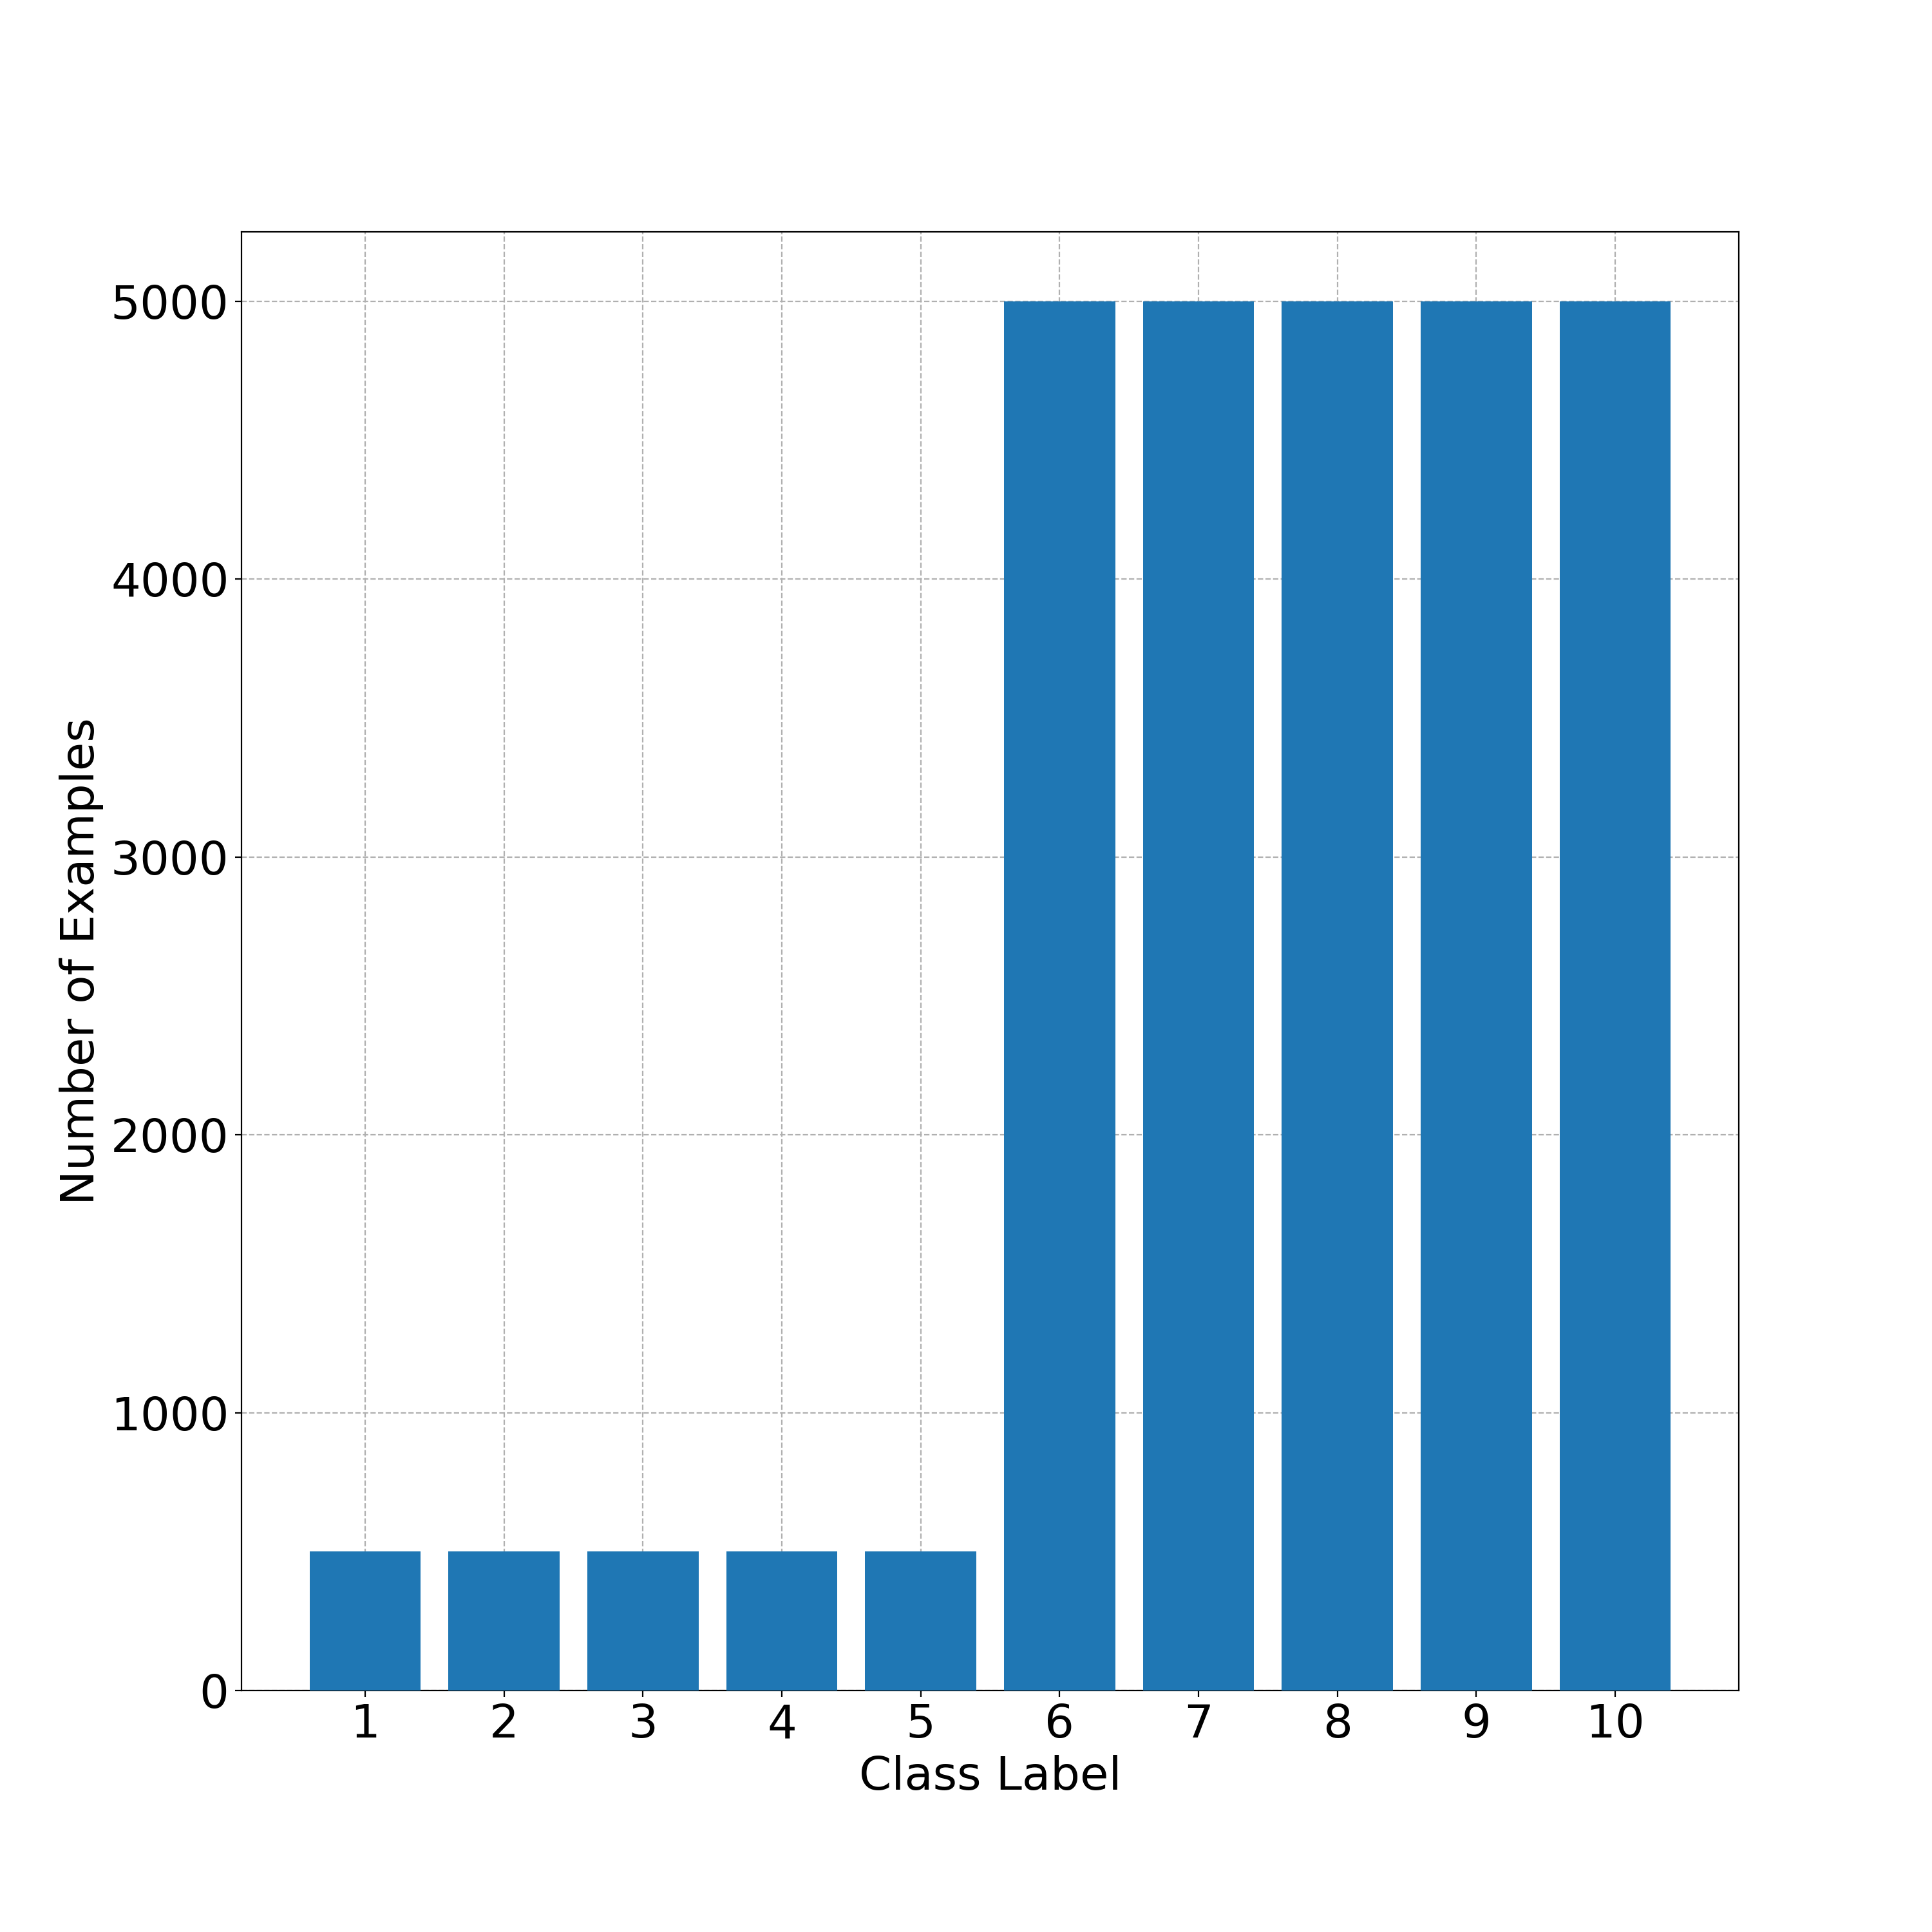
\includegraphics[width=0.45\columnwidth]{imbalance-distribution-1}
      \label{fig:imb-dist:1}
  }
  \subfigure[]{
      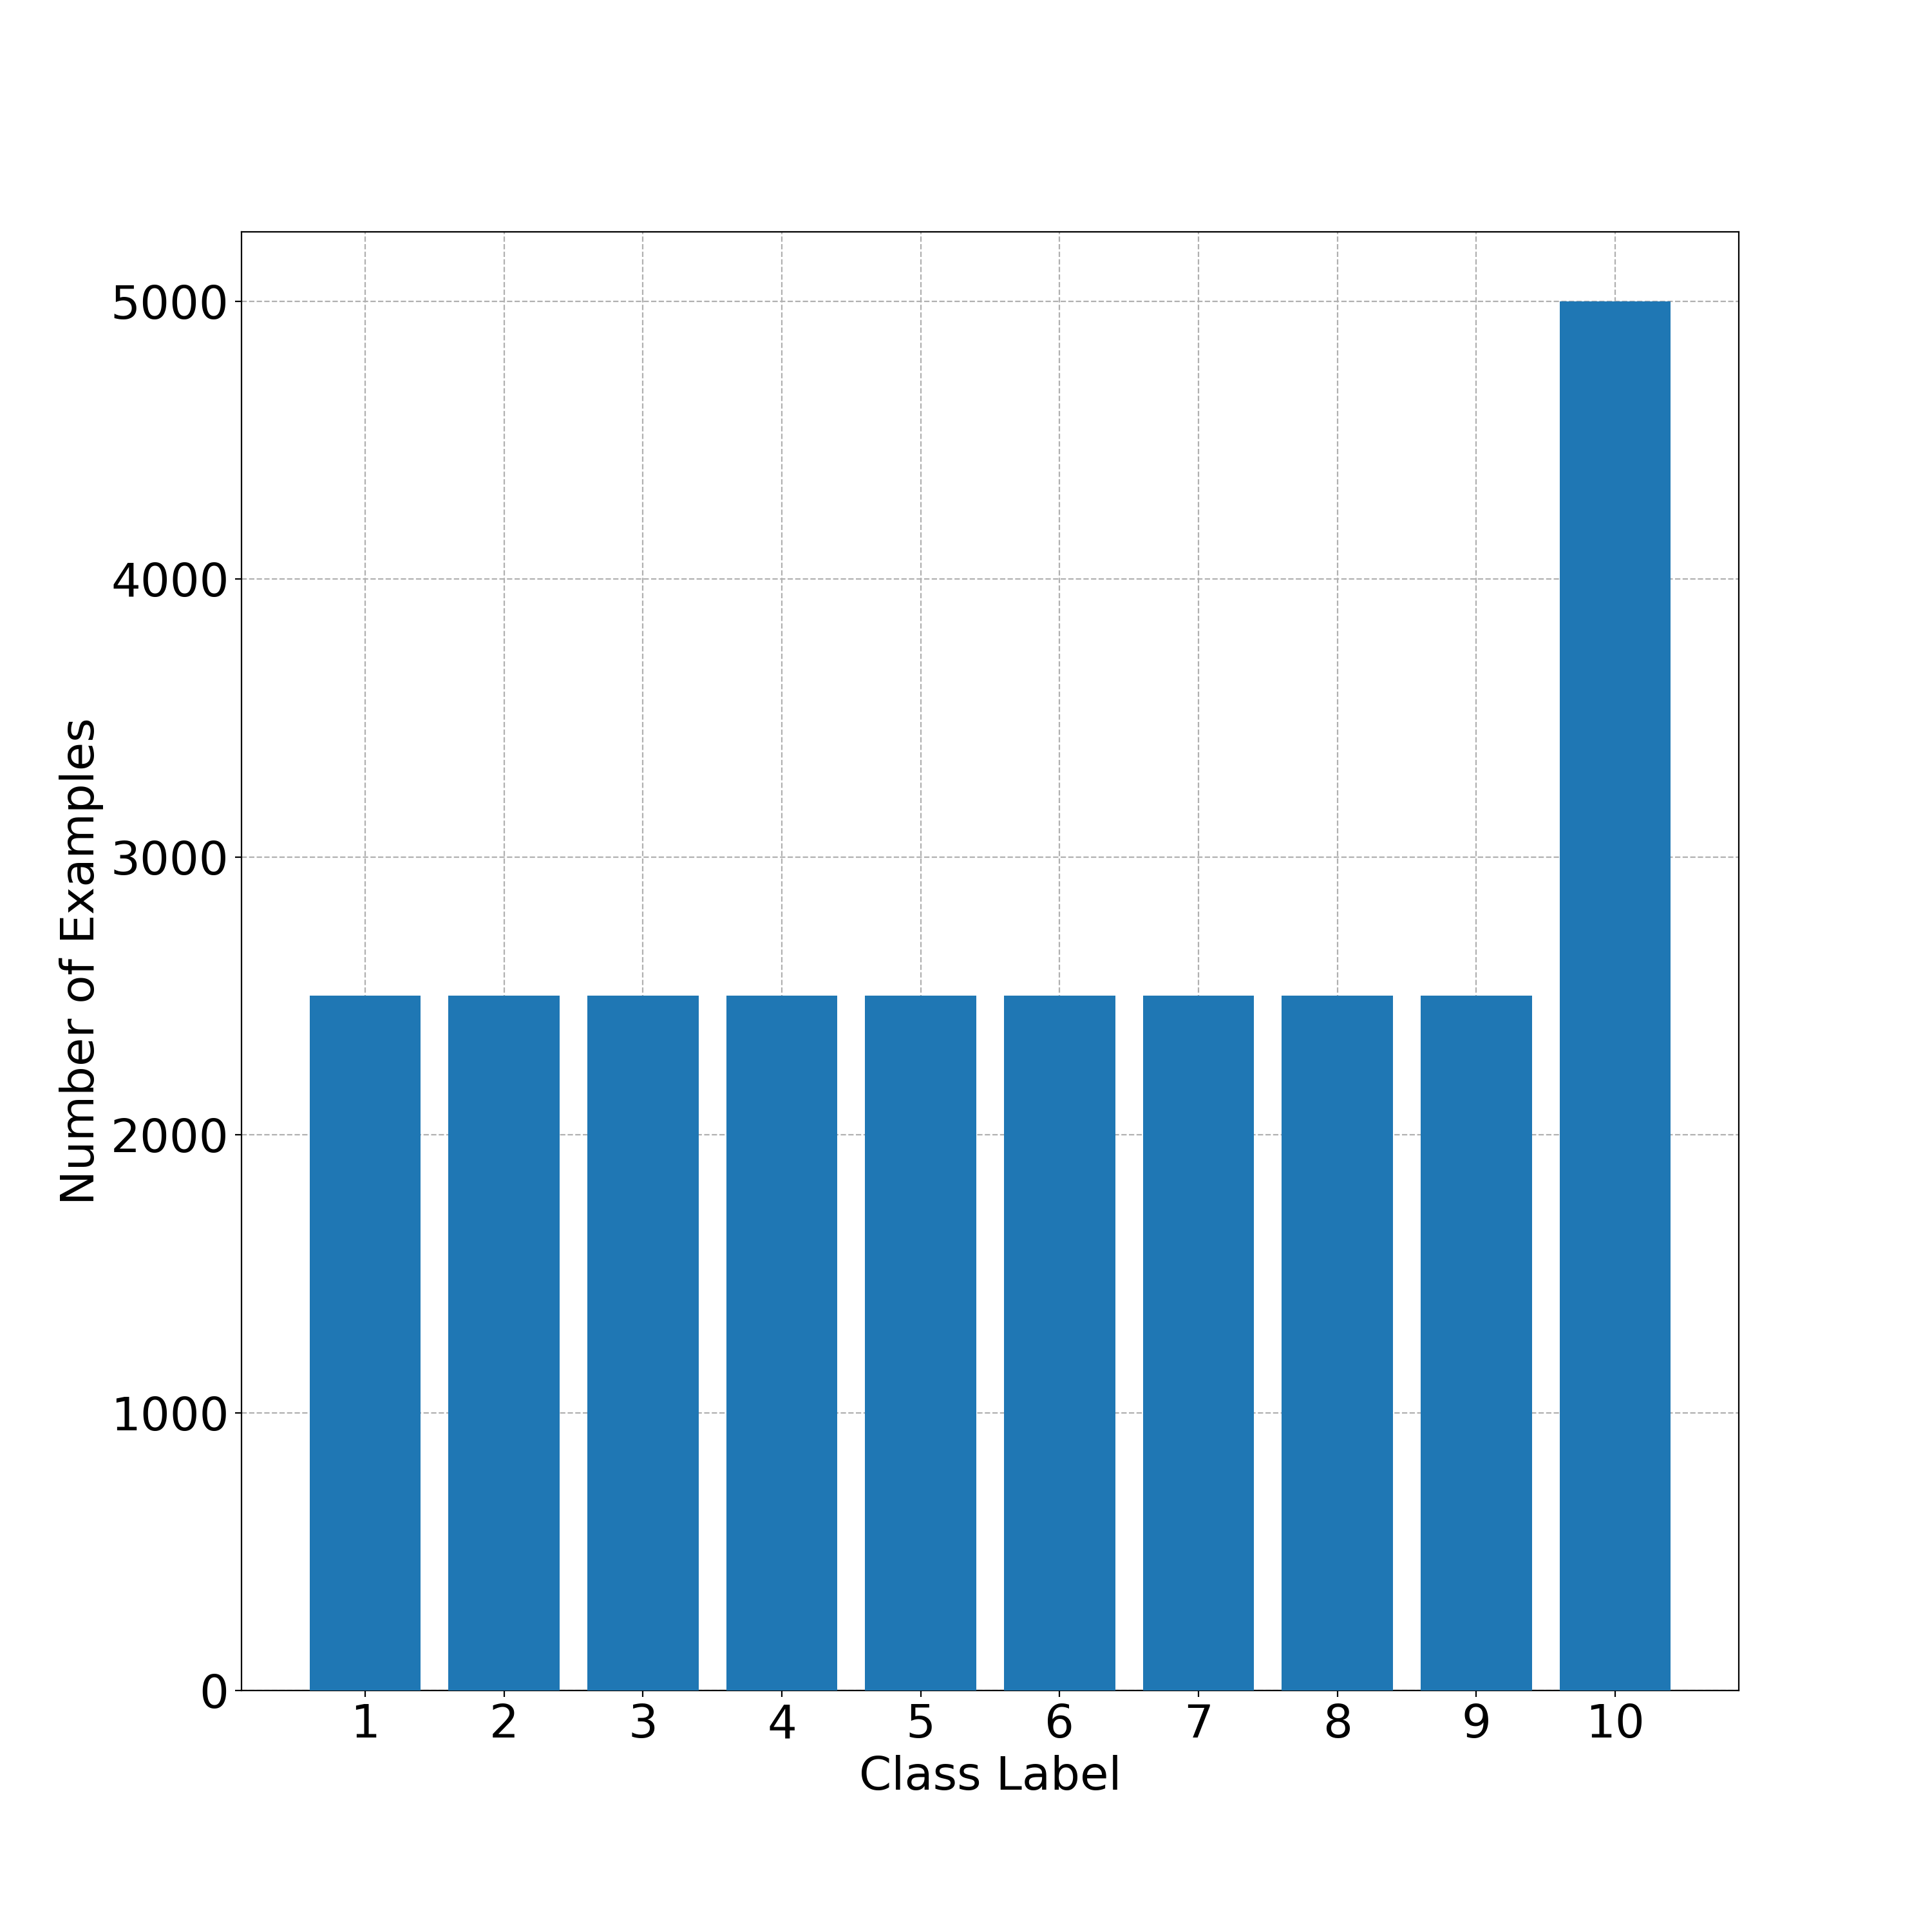
\includegraphics[width=0.45\columnwidth]{imbalance-distribution-2}
      \label{fig:imb-dist:2}
  }
  \subfigure[]{
    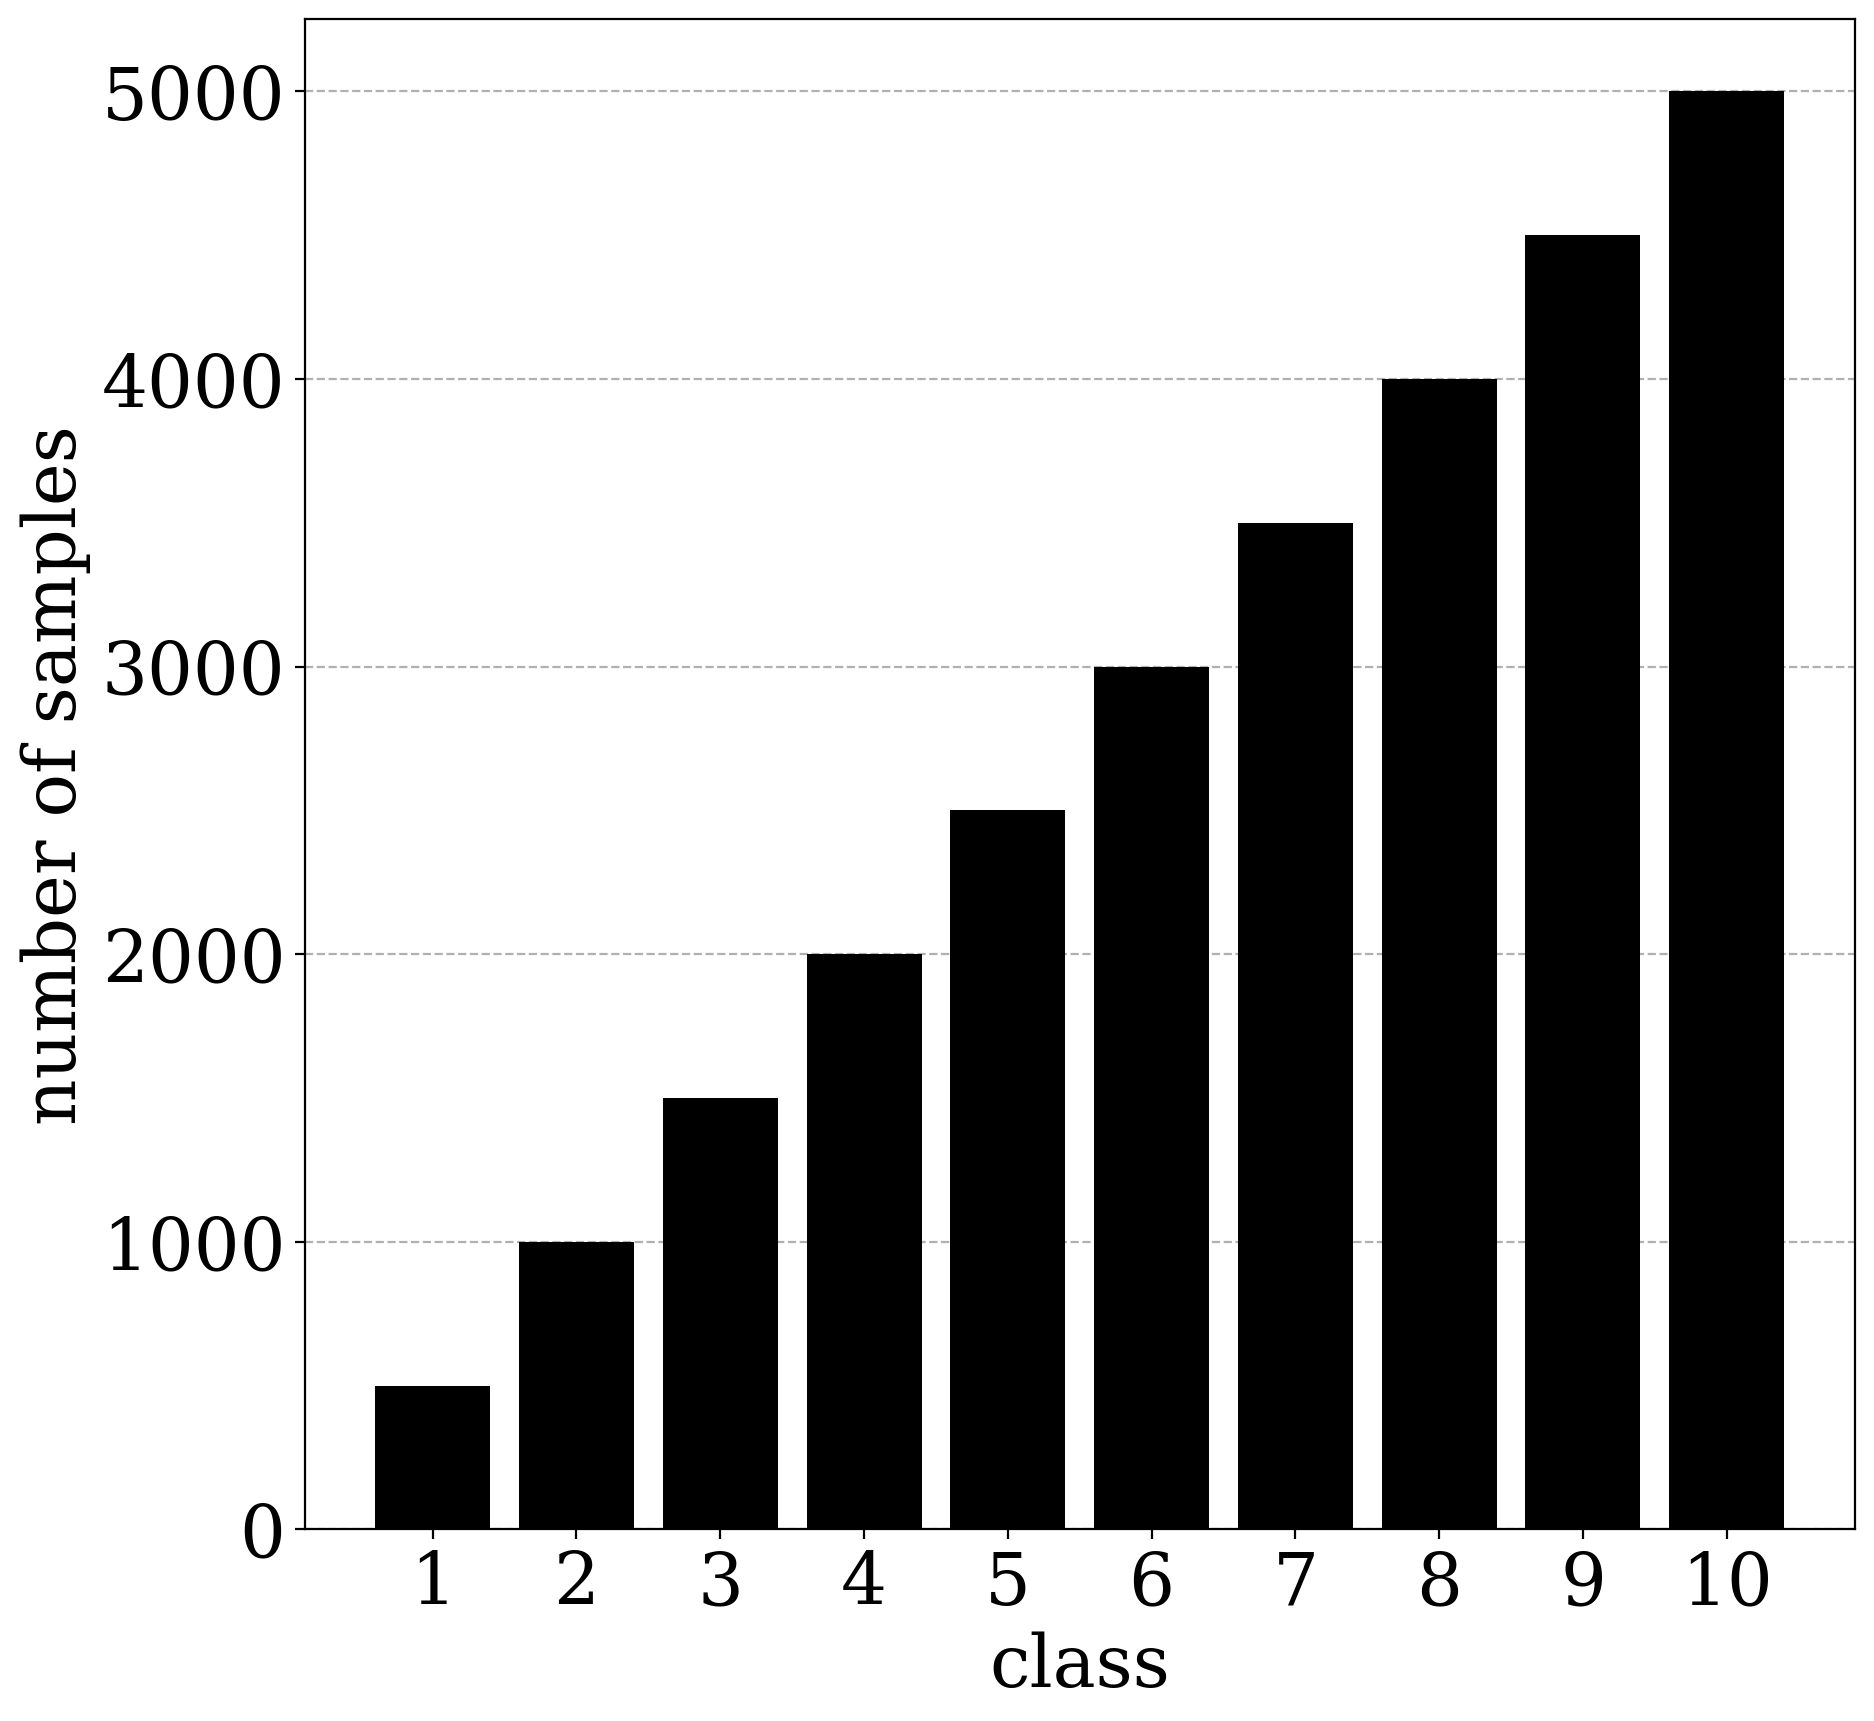
\includegraphics[width=0.45\columnwidth]{imbalance-distribution-3}
    \label{fig:imb-dist:3}
  }
  \caption{ตัวอย่างการกระจายของจำนวนตัวอย่างของกลุ่มข้อมูล (ก) $p = 10$, $\mu = 0.5$ (ข) $p = 2$, $\mu = 0.9$ (ค) $p = 10$}
  \label{fig:imb-dist}
\end{figure}
\FloatBarrier

\subsection{การจัดการปัญหาความไม่สมดุลกันของกลุ่มข้อมูลด้วยวิธีการต่าง ๆ}
\subsubsection{Cost-Sensitive Learning}
Cost-Sensitive Learning เป็นหนึ่งในเทคนิคการเรียนรู้ของอัลกอริทึมการจัดกลุ่มข้อมูลที่มีการนำ ค่าความเสียหายของการระบุกลุ่มข้อมูลผิดพลาด (Misclassification Cost) มาพิจารณาเพื่อที่จะพยายามลดค่าความเสียหายดังกล่าวให้น้อยที่สุด~\cite{Ling-CS:2010} 
ในกระบวนการเรียนรู้ของอัลกอริทึมการจัดกลุ่มข้อมูล ส่วนใหญ่พยายามที่จะลดอัตราความผิดพลาดในการระบุกลุ่มข้อมูลให้น้อยที่สุด ซึ่งอัตราความผิดพลาด คือ อัตราของการระบุกลุ่มข้อมูลผิด 
โดยแบ่งออกเป็นสองประเภท คือ ความผิดพลาดที่ระบุข้อมูลกลุ่ม Positive เป็นกลุ่ม Negative (False Negative) และ ความผิดพลาดที่ระบุข้อมูลกลุ่ม Negative เป็นกลุ่ม Positive (False Positive) 
อัลกอริทึมดังกล่าวจะพยายามลดความผิดพลาดโดยรวม กล่าวคือ ให้ความสำคัญที่ False Negative และ False Positive เท่ากัน

ในความเป็นจริงบางครั้งความผิดพลาดดังกล่าวไม่ควรให้ความสำคัญเท่ากัน เช่น ในการตรวจวินิฉัยโรคมะเร็ง ที่ซึ่งผู้ป่วยที่มีโรคมะเร็งเป็นข้อมูลกลุ่ม Positive และผู้ป่วยที่มีสุขภาพดีเป็นข้อมูลกลุ่ม Negative 
การวินิจฉัยผิดพลาดว่าผู้ป่วยมีสุขภาพดี แต่จริง ๆ แล้วมีโรคมะเร็ง (False Negative) นั้นมีความเสียหายมากกว่าการที่วินิจฉัยผิดพลาดว่าผู้ป่วยมีโรคมะเร็ง แต่จริง ๆ แล้วมีสุขภาพดี (False Positive) ดังนั้นควรจะให้ความสำคัญที่ False Negative มากกว่า เป็นต้น 

Cost-Sensitive Learning จะให้ความสำคัญกับความเสียหายดังกล่าวไม่เท่ากัน ที่ซึ่ง False Negative จะถูกให้ความสำคัญมากกว่า และเรียกว่าเป็นค่าความเสียหายของการระบุกลุ่มข้อมูลผิดพลาด ค่าความเสียหายถูกระบุไว้ดังตารางที่ \ref{table:2:cost-matrix} ซึ่งเรียกว่า Cost Matrix โดยที่ C(i,j) คือ ค่าความเสียหายในการระบุข้อมูลกลุ่ม j เป็นกลุ่ม i

โดยปกติแล้ว Cost-Sensitive ถูกนำมาใช้ในการแก้ปัญหาความไม่สมดุลกันของข้อมูล เนื่องจาก โดยทั่วไปกลุ่มข้อมูลส่วนใหญ่นั้นจะเป็นกลุ่ม Positive และข้อมูลกลุ่ม Positive มักจะถูกระบุผิดว่าเป็นกลุ่ม Negative

\begin{table}[]
	\caption{ตัวอย่างของ Cost Matrix สำหรับการจัดกลุ่มข้อมูลสองกลุ่ม โดย 1 คือ Positive และ 0 คือ Negative}
	\label{table:2:cost-matrix}
	\centering
  \begin{tabular}{l|l|l|}
    \cline{2-3}
     & \textbf{Actual Negative} & \textbf{Actual Positive} \\ \hline
    \multicolumn{1}{|l|}{Predict Negative} & C(0,0), or TP & C(0,1), or \emph{FN} \\ \hline
    \multicolumn{1}{|l|}{Predict Positive} & C(1,0), or \emph{FP} & C(1,1), or TP \\ \hline
    \end{tabular}
\end{table}
\FloatBarrier

\subsection{การเรียนรู้เชิงลึก (Deep Learning)}
Ian Goodfellow et al. \cite{Goodfellow:2016} ได้อธิบายว่า การเรียนรู้เชิงลึกเป็นวิธีการที่สามารถแก้ปัญหาที่ดำเนินการได้ง่ายสำหรับมนุษย์ แต่ยากต่อการอธิบาย 
กล่าวคือ ปัญหาเหล่านั้นเป็นปัญหาที่เราสามารถแก้ได้อย่างอัตโนมัตด้วยสัญชาตญาณ  เช่น การจดจำคำพูด หรือใบหน้าผู้คนในรูป เป็นต้น 
สามารถเรียกปัญหาหรืองานประเภทนี้ว่า งานที่เป็นรูปแบบ (Formal Task) ในทางตรงกันข้าม ปัญหาหรืองานที่ไม่เป็นรูปแบบ (Informal Task) 
ที่ซึ่งยากสำหรับมนุษย์ในการดำเนินการ แต่ง่ายสำหรับการประมวลของคอมพิวเตอร์ ปัญหาประเภทนี้จะสามารถถูกอธิบายออกมาในรูปแบบของสมการคณิตศาสตร์ 
หรือมีวิธีการคำนวณทางคณิตศาสตร์ได้ เช่น การพยากรณ์สภาพอากาศ ที่ซึ่งปัจจัยต่าง ๆ ที่เกี่ยวข้อง อย่าง ค่าความชื้น ค่าอุณหภูมิวันก่อนหน้า และค่าอื่น ๆ 
จะถูกนำมาคำนวณ เป็นต้น

การเรียนรู้เชิงลึกทำให้คอมพิวเตอร์สามารถเรียนรู้จากประสบการณ์ และเข้าใจสิ่งต่าง ๆ แบบเป็นลำดับชั้นของแนวคิดเหมือนกับมนุษย์ 
โดยที่แต่ละลำดับชั้นของแนวคิดถูกกำหนดผ่านความสัมพันธ์กับชั้นของแนวคิดที่ไม่ซับซ้อน กล่าวคือ 
แนวคิดที่เป็นลำดับชั้นทำให้คอมพิวเตอร์สามารถเรียนรู้แนวคิดที่ซับซ้อนโดยการสร้างมันจากแนวคิดที่ไม่ซับซ้อน 

ในศาสตร์ทางด้านปัญญาประดิษฐ์ (Artificial Intelligence: AI) การที่ระบบคอมพิวเตอร์สามารถได้รับมาซึ่งความรู้จากการสกัดรูปแบบของข้อมูลดิบ 
เรียกความสามารถนี้ว่า การเรียนรู้ของเครื่องจักร อัลกอริธึมพื้นฐานของการเรียนรู้ของเครื่องจักรอย่าง Logistic Regression 
Linear Regression หรือ Naive Bayes สามารถประมวลเพื่อดำเนินงานที่เป็นรูปแบบต่าง ๆ เช่น พยากรณ์สภาพอากาศ 
แนะนำช่วงเวลาสำหรับการคลอดลูก หรือแยกแยะอีเมลที่ถูกต้องออกจากอีเมลขยะ เป็นต้น ประสิทธิภาพของอัลกอริธึมพื้นฐานเหล่านั้นขึ้นอยู่กับคุณลักษณะ (Feature) ของข้อมูลที่ได้รับ ตัวอย่างเช่น เมื่อการถดถอยโลจิสติกส์ถูกใช้ในการพยากรณ์โรคมะเร็งเต้านม หมอจะต้องให้ข้อมูลที่เกี่ยวข้องแก่อัลกอริธึม 
เช่น เต้านมมีผื่น แดง ร้อน ผื่นคล้ายผิวส้มหรือไม่ และมีก้อนหนาๆ ในเต้านมหรือใต้แขนหรือไม่ เป็นต้น ข้อมูลดังกล่าวเป็นคุณลักษณะของคนไข้ 
ซึ่งเรียกแต่ละประเภทข้อมูลว่า คุณลักษณะ การถดถอยโลจิสติกส์จะเรียนรู้ว่าคุณลักษณะเหล่านั้นมีความสัมพันธ์กันอย่างไรกับผลลัพธ์ ซึ่งผลลัพธ์ในตัวอย่างนี่คือ 
โอกาสในการเป็นโรคมะเร็งเต้านม อย่างไรก็ตามอัลกอริธึมไม่สามารถกำหนดได้ว่าคุณลักษณะต้องถูกกำหนดมาอย่างไร กล่าวคือ 
การได้มาซึ่งค่าของคุณลักษณะไม่ใช่หน้าที่ของอัลกอริทึม เพราะฉะนั้นถ้าอัลกอริธึมได้รับภาพ MRI มาเพื่อพยากรณ์โรคมะเร็งเต้านม แทนการใช้ข้อมูลที่เป็นรูปแบบของหมอ 
จะทำอัลกอริธีมไม่สามารถพยากรณ์ผลลัพธ์ที่เป็นประโยชน์ได้ หรือผลลัพธ์ที่ได้จะไม่น่าเชื่อถือเลย เพราะค่า Pixel ในภาพ MRI 
ไม่ได้มีความสัมพันธ์กันกับลักษณะความผิดปกติของเต้านมอย่างสิ้นเชิง

แบบจำลองพื้นฐานของการเรียนรู้เชิงลึก คือ Multi-Layer Perceptron (MLP) ที่ซึ่งเป็นเพียงฟังก์ชันคณิตศาสตร์ที่ทำการแปลงค่าข้อมูลขาเข้าไปเป็นข้อมูลขาออก ฟังก์ชันจะถูกสร้างขึ้นจากการประกอบเข้าด้วยกันของหลายฟังก์ชันที่เป็นพื้นฐานกว่า 
เราสามารถใช้ฟังก์ชันที่ต่างกันในแต่ละงานเพื่อให้ได้มาซึ่งคุณลักษณะของข้อมูลที่เหมาะสมกับงานนั้น ๆ

\subsection{การเรียนรู้ของโมเดล Deep Learning}
\subsection{ฟังก์ชันสูญเสีย (Loss Function)}

\section{งานวิจัยที่เกี่ยวข้อง}
เมื่อเทคนิคการจัดกลุ่มข้อมูลที่ประกอบด้วยโครงข่ายประสาทแบบคอนโวลูชันถูกใช้กับชุดข้อมูลที่มีความไม่สมดุลกัน อัตราการพยากรณ์ผิดพลาดจะมีค่าสูงเมื่อเทียบกับการเพิ่มขึ้นของจำนวนรอบของการเรียนรู้ของแบบจำลอง กล่าวคือ ยิ่งจำนวนรอบของการเรียนรู้สูงขึ้น จะทำให้อัตราการพยากรณ์ผิดพลาดสูงขึ้นด้วย \cite{Yan:2015} เบื้องหลังของสาเหตุที่ทำให้เป็นเช่นนั้น คือ ในเสตจของการเรียนรู้ของแบบจำลองการเรียนรู้เชิงลึก ข้อมูลจะถูกแบ่งออกเป็นกลุ่ม ๆ ซึ่งทำให้แต่ละกลุ่มมีความไม่เท่าเทียมกันเมื่อข้อมูลไม่สมดุลกัน อีกทั้งบางกลุ่มอาจจะมีแค่ตัวอย่างของกลุ่มข้อมูลที่เป็นส่วนมาก หรือกลุ่มข้อมูลที่เป็นส่วนน้อยเท่านั้น เมื่อแบบจำลองได้เรียนรู้ข้อมูลจากกลุ่มเหล่านั้นในทุก ๆ รอบ จึงทำให้เกิดอัตราการพยากรณ์ผิดพลาดที่สูง

เมื่อไม่นานมานี้ได้มีงานวิจัยที่พยายามจัดการกับปัญหาการเรียนรู้ของแบบจำลองการเรียนรู้เชิงลึกเมื่อต้องเรียนรู้ข้อมูลที่มีความไม่สมดุลกัน ดังต่อไปนี้